% Chapter 12, Section 3

\section{Speech Recognition and Synthesis \difficultyInline{beginner}}
\label{sec:speech-applications}

Speech recognition and synthesis represent one of the most transformative applications of deep learning, enabling natural human-computer interaction through voice interfaces. These technologies have revolutionized how we interact with devices, from smartphones and smart speakers to automotive systems and accessibility tools. The field has evolved from rule-based systems to end-to-end neural architectures that can understand and generate human speech with remarkable accuracy and naturalness. Modern speech systems power virtual assistants, real-time translation services, and assistive technologies that improve accessibility for millions of users worldwide. The integration of self-supervised learning and transformer architectures has further enhanced the robustness and multilingual capabilities of these systems, making them essential components of modern AI applications.

\subsection{Automatic Speech Recognition (ASR)}

Automatic Speech Recognition (ASR) converts spoken language into text, serving as the foundation for voice-controlled applications and accessibility tools. Modern ASR systems use deep neural networks to process audio signals, extracting meaningful text from speech with high accuracy across diverse languages and accents. The technology has evolved from simple command recognition to sophisticated systems that can handle continuous speech, multiple speakers, and noisy environments. Self-supervised pretraining techniques like wav2vec have significantly reduced the need for large amounts of labeled data, making ASR more accessible and cost-effective. These systems are now integrated into everyday applications, from virtual assistants and transcription services to real-time translation and voice commands in smart devices.

Virtual assistants like Siri, Alexa, and Google Assistant have become ubiquitous in modern life, providing hands-free access to information, entertainment, and smart home control. These systems use advanced ASR to understand natural language commands, enabling users to set reminders, play music, control lighting, and access weather information through simple voice interactions. The technology has transformed how we interact with technology, making it more accessible to users with mobility limitations and providing convenience in situations where hands-free operation is essential. These assistants continue to evolve, incorporating more sophisticated language understanding and context awareness to provide increasingly natural and helpful interactions.

Transcription services have revolutionized documentation and accessibility, converting spoken content into text for meetings, lectures, interviews, and media content. Professional transcription services use advanced ASR to provide accurate, real-time transcription for legal proceedings, medical consultations, and educational content. The technology has made information more accessible to deaf and hard-of-hearing individuals, enabling them to participate fully in conversations and access audio content. Real-time transcription services are now integrated into video conferencing platforms, providing live captions for remote meetings and webinars, enhancing accessibility and comprehension for all participants.

Voice commands have transformed user interfaces across multiple domains, enabling hands-free control of devices and applications. In automotive systems, voice commands allow drivers to control navigation, make phone calls, and adjust settings without taking their hands off the wheel, improving safety and convenience. Smart home systems use voice commands to control lighting, temperature, security systems, and entertainment devices, creating seamless and intuitive living environments. The technology has also found applications in healthcare, where voice commands enable hands-free operation of medical equipment, reducing the risk of contamination and improving workflow efficiency in sterile environments.

The architectures used in modern ASR systems have evolved significantly, with CTC-based models providing efficient training for sequence-to-sequence tasks by allowing flexible alignment between audio and text. Listen-Attend-Spell architectures use attention mechanisms to focus on relevant parts of the audio signal, improving accuracy for long sequences and complex utterances. Transducer models combine the benefits of CTC and attention-based approaches, providing both efficiency and accuracy for real-time applications. Self-supervised pretraining with models like wav2vec has revolutionized the field by learning rich audio representations from unlabeled data, reducing the need for expensive labeled datasets and improving performance on low-resource languages and domains.

\begin{figure}[h]
  \centering
  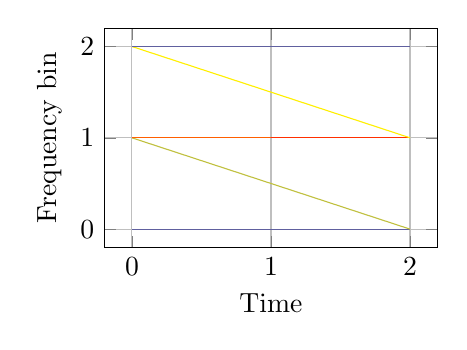
\begin{tikzpicture}
    \begin{axis}[
      width=0.48\textwidth,height=0.36\textwidth,
      xlabel={Time}, ylabel={Frequency bin}, grid=both]
      \addplot[mesh,draw=none,shader=interp,point meta=explicit] coordinates{ (0,0) [0.1] (1,0) [0.2] (2,0) [0.1]
        (0,1) [0.3] (1,1) [0.5] (2,1) [0.4]
        (0,2) [0.1] (1,2) [0.2] (2,2) [0.1] };
    \end{axis}
  \end{tikzpicture}
  \caption{Schematic spectrogram input for ASR.}
  \label{fig:asr-spec}
\end{figure}

\subsection{Text-to-Speech (TTS)}

Text-to-Speech (TTS) technology converts written text into natural-sounding speech, enabling applications that require audio output from text content. Modern TTS systems use neural vocoders and advanced synthesis techniques to generate speech that is virtually indistinguishable from human speech in terms of naturalness and expressiveness. The technology has evolved from robotic-sounding concatenative synthesis to sophisticated neural approaches that can capture the nuances of human speech, including emotion, intonation, and prosody. TTS systems are now integrated into a wide range of applications, from accessibility tools and virtual assistants to entertainment and educational content, making information more accessible and engaging for users with visual impairments or learning preferences.

WaveNet and Tacotron represent breakthrough architectures in neural TTS, using deep learning to generate high-quality speech from text input. WaveNet uses dilated convolutions to model the temporal dependencies in speech, producing more natural-sounding audio with better prosody and expressiveness. Tacotron combines sequence-to-sequence learning with attention mechanisms to generate mel-spectrograms from text, which are then converted to audio using neural vocoders. These architectures have enabled the development of voice synthesis systems that can mimic specific speakers, create custom voices for applications, and generate speech in multiple languages with native-like pronunciation. The technology has found applications in audiobook production, virtual assistants, and personalized voice interfaces.

Voice cloning technology has emerged as a powerful application of TTS, enabling the creation of synthetic voices that closely mimic specific individuals. This technology has applications in entertainment, where it can be used to create voiceovers for characters or restore the voices of actors who have passed away. In accessibility, voice cloning can help individuals with speech impairments create personalized synthetic voices that sound more natural and expressive than traditional text-to-speech systems. The technology has also found applications in language learning, where learners can practice pronunciation with native speaker voices, and in customer service, where synthetic voices can provide consistent and professional interactions. However, the technology also raises important ethical considerations regarding consent, privacy, and the potential for misuse in creating deepfake audio content.

Accessibility tools powered by TTS technology have transformed the lives of individuals with visual impairments, learning disabilities, and other conditions that affect reading ability. Screen readers use TTS to convert digital text into speech, enabling blind and visually impaired users to access websites, documents, and applications independently. Educational TTS systems can read textbooks, articles, and other learning materials aloud, supporting students with dyslexia and other reading difficulties. The technology has also enabled the creation of audiobooks and spoken content for entertainment and education, making information more accessible to diverse audiences. These tools continue to evolve, incorporating more natural-sounding voices, better pronunciation of technical terms, and support for multiple languages and accents.

\subsection{Speaker Recognition}

Speaker recognition technology identifies and verifies individuals based on their unique vocal characteristics, providing secure and convenient authentication methods. The technology analyzes various acoustic features of speech, including pitch, formants, and spectral characteristics, to create unique voiceprints for each individual. Modern speaker recognition systems use deep learning approaches to extract robust features that are resistant to noise, aging, and other factors that might affect voice quality. The technology has applications in security, authentication, and personalization, enabling hands-free access to devices and services. Speaker recognition is also used in forensic applications, where it can help identify individuals from audio recordings in criminal investigations.

Voice biometrics use speaker recognition technology to provide secure authentication for banking, healthcare, and other sensitive applications. Banks and financial institutions use voice biometrics to verify customer identity during phone calls, reducing fraud and improving security while maintaining convenience. Healthcare systems use voice authentication to secure access to patient records and medical devices, ensuring that only authorized personnel can access sensitive information. The technology has also found applications in smart home security, where it can recognize authorized users and grant access to restricted areas or functions. Voice biometrics offer several advantages over traditional authentication methods, including hands-free operation, resistance to spoofing attacks, and the ability to work across different devices and platforms.

Speaker diarization technology identifies who spoke when in multi-speaker conversations, providing valuable insights for meeting analysis, transcription, and content organization. The technology uses machine learning algorithms to segment audio recordings by speaker, enabling automatic identification of different participants in conversations. This capability is essential for accurate transcription of meetings, interviews, and other multi-speaker events, where it's important to know which person said what. Speaker diarization is also used in call center analytics, where it can help identify customer service representatives and customers in recorded calls for quality assurance and training purposes. The technology has applications in media production, where it can automatically identify and label different speakers in podcasts, interviews, and other audio content.

\subsection{Historical context and references}

The development of speech recognition and synthesis has been marked by several key breakthroughs that have transformed the field from rule-based systems to sophisticated neural architectures. The introduction of Hidden Markov Models (HMMs) in the 1970s provided the first statistical approach to speech recognition, enabling systems to learn from data rather than relying on hand-crafted rules. The development of Mel-Frequency Cepstral Coefficients (MFCCs) in the 1980s provided robust feature extraction methods that became the standard for speech processing systems. The introduction of neural networks in the 1990s marked a significant shift, with systems like TIMIT demonstrating the potential of deep learning for speech recognition tasks.

The 2000s saw the development of more sophisticated neural architectures, including Long Short-Term Memory (LSTM) networks and attention mechanisms that improved the ability to handle long sequences and complex speech patterns. The introduction of Connectionist Temporal Classification (CTC) in 2006 provided an efficient method for training sequence-to-sequence models without requiring frame-level alignments, making it easier to train ASR systems on large datasets. The development of WaveNet in 2016 marked a breakthrough in neural TTS, demonstrating that deep learning could generate high-quality speech that was virtually indistinguishable from human speech. The introduction of transformer architectures in 2017 further revolutionized the field, enabling more efficient processing of sequential data and better capture of long-range dependencies in speech.

The 2020s have seen the integration of self-supervised learning and large-scale pretraining, with models like wav2vec and Whisper demonstrating the power of learning from unlabeled audio data. These developments have made speech technology more accessible and cost-effective, enabling the development of systems that can work across multiple languages and domains with minimal labeled data. The field continues to evolve rapidly, with new architectures, training methods, and applications emerging regularly, making speech recognition and synthesis one of the most dynamic and impactful areas of artificial intelligence. See \textcite{Prince2023} for broader context and comprehensive tutorials on the theoretical foundations and practical applications of these transformative technologies.

